
$\triangle ABC$ and $\triangle DBC$ are two isosceles triangles on the same base $BC$ and the vertices $A$ and $D$ are on the same side of $BC$. If $AD$ is extended to intersect $BC$ at $P$, show that \\
a) $\triangle ABD$ $\cong$ $\triangle ACD$ \\
b) $\triangle ABP$ $\cong$ $\triangle ACP$ \\
c) $AP$ bisects $\angle A$ as well as $\angle D$\\
d) $AP$ is the parpendicular bisector of $BC$

\begin{figure}[!ht]
\centering
\resizebox{\columnwidth}{!}{%\documentclass{standalone}
%
%\usepackage{tikz,pgf} %and any other packages or tikzlibraries your picture needs
%
%\begin{document}
%\resizebox{\columnwidth}{!}{
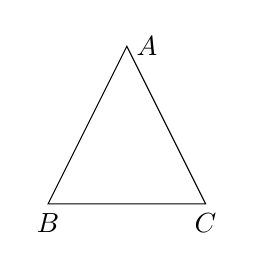
\begin{tikzpicture}
\draw (0,0) node[anchor=north]{$B$}
  -- (1,2) node[anchor=west]{$A$}
  -- (2,0) node[anchor=north]{$C$}
  -- cycle;
\end{tikzpicture}
%}
%\end{document}}
\caption{Iso-sceles Triangles by Latex-Tikz}
\label{eq:solutions/1/33/fig:iso_scelen}	
\end{figure}

The above problem statement is depicted in the figure \ref{eq:solutions/1/33/fig:iso_scelen} where the vertices are: A, B and C for $\triangle ABC$ and D, B and C for $\triangle DBC$. For $\triangle ABC$ the sides AB, BC and CA are represented by the vectors $\vec{A-B}$ , $\vec{B-C}$ and $\vec{C-A}$ and for $\triangle DBC$ the sides DB, BC and CD are represented by $\vec{D-B}$ , $\vec{B-C}$ and $\vec{C-D}$.

From the problem statement we get that:
\begin{equation}
\begin{aligned}
\norm{\vec{A}-\vec{B}} = \norm{\vec{A}-\vec{C}}
%\implies \norm{\vec{AB}} = \norm{\vec{AC}}
\end{aligned}
\end{equation}
\label{eq:solutions/1/33/cond1}
\begin{align}
\norm{\vec{D}-\vec{B}} = \norm{\vec{D}-\vec{C}}
%\implies \norm{\vec{DB}} = \norm{\vec{DC}}
\end{align}
\label{eq:solutions/1/33/cond2}
\begin{align}
\vec{P-C} = K_2 (\vec{B-C})\\
\vec{P-B} = K_1 (\vec{B-C})
\end{align}
\begin{multline}
\norm{\vec{A-B}} = \norm{\vec{A}-\vec{C}}\\
\implies \norm{\vec{A-B}}^2 = \norm{\vec{A-C}}^2\\
\implies \norm{{(\vec{A-P}) + (\vec{P-B})}}^2 = \norm{{(\vec{A-P}) + (\vec{P-C})}}^2\\
\implies \norm{\vec{A-P}}^2 + \norm{\vec{P-B}}^2 + 2(\vec{A-P})^T (\vec{P-B})=\\
\norm{\vec{A-P}}^2 + \norm{\vec{P-C}}^2 + 2(\vec{A-P})^T (\vec{P-C})\\
\implies \norm{\vec{P-B}}^2 + 2(\vec{A-P})^T (\vec{P-B})=\\
\norm{\vec{P-C}}^2 + 2(\vec{A-P})^T (\vec{P-C})\\
\implies \norm{\vec{P-B}}^2 -\norm{\vec{P-C}}^2\\
 + 2(\vec{A-P})^T ((\vec{P-B})-(\vec{P-C})) =0\\
\implies ((\vec{P-B})+(\vec{P-C}))^T ((\vec{P-B})-(\vec{P-C}))\\
+ 2(\vec{A-P})^T ((\vec{P-B})-(\vec{P-C})) =0\\
\implies (\vec{B}+\vec{C}-2\vec{P})^T (\vec{B-C})\\
+2(\vec{A-P})^T (\vec{P}-\vec{B}-\vec{P}+\vec{C}) =0\\
\implies (\vec{B}+\vec{C}-2\vec{P})^T (\vec{B-C})+2(\vec{A-P})^T (\vec{B-C}) =0\\
\implies ((\vec{B}+\vec{C}-2\vec{P})^T - 2(\vec{A-P})^T)(\vec{B-C})=0\\
\implies ((\vec{B}+\vec{C}-2\vec{P})-(\vec{2A-2P}))^T (\vec{B-C})=0\\
\implies (\vec{B+C-2A})^T (\vec{B-C})=0\\
\implies (\vec{B-C})^T (\vec{B+C-2A})=0\\
\label{eq:solutions/1/33/cond3}
\end{multline}
Now, from \ref{eq:solutions/1/33/cond3}
\begin{multline}
(\vec{B-C})^T \brak{\vec{\brak{\frac{B+C}{2}}-A}}=0\\
\implies \brak{\vec{\brak{\frac{B+C}{2}}-A}} \perp (\vec{B-C})
\end{multline}
So, we can conclude that $\vec{A-P}$ bisects $\vec{B-C}$ perpendicularly.
Similarly, 
\begin{multline}
\norm{\vec{D-B}} = \norm{\vec{D-C}}\\
\implies \norm{\vec{D-B}}^2 = \norm{\vec{D-C}}^2\\
\implies \norm{{(\vec{D-P}) + (\vec{P-B})}}^2 = \norm{{(\vec{D-P}) + (\vec{P-C})}}^2\\
\implies \norm{\vec{D-P}}^2 + \norm{\vec{P-B}}^2 + 2(\vec{D-P})^T (\vec{P-B})=\\
\norm{\vec{D-P}}^2 + \norm{\vec{P-C}}^2 + 2(\vec{D-P})^T (\vec{P-C})\\
\implies \norm{\vec{P-B}}^2 + 2(\vec{D-P})^T (\vec{P-B})=\\
\norm{\vec{P-C}}^2 + 2(\vec{D-P})^T (\vec{P-C})\\
\implies \norm{\vec{P-B}}^2 -\norm{\vec{P-C}}^2\\
 + 2(\vec{D-P})^T ((\vec{P-B})-(\vec{P-C})) =0\\
\implies ((\vec{P-B})+(\vec{P-C}))^T ((\vec{P-B})-(\vec{P-C}))\\
+ 2(\vec{D-P})^T ((\vec{P-B})-(\vec{P-C})) =0\\
\implies (\vec{B}+\vec{C}-2\vec{P})^T (\vec{B-C})\\
+2(\vec{D-P})^T (\vec{P}-\vec{B}-\vec{P}+\vec{C}) =0\\
\implies (\vec{B}+\vec{C}-2\vec{P})^T (\vec{B-C})+2(\vec{D-P})^T (\vec{B-C}) =0\\
\implies ((\vec{B}+\vec{C}-2\vec{P})^T - 2(\vec{D-P})^T) (\vec{B-C})=0\\
\implies ((\vec{B}+\vec{C}-2\vec{P})-(\vec{2D-2P}))^T (\vec{B-C})=0\\
\implies (\vec{B+C-2D})^T (\vec{B-C})=0\\
\implies (\vec{B-C})^T (\vec{B+C-2D})=0\\
\label{eq:solutions/1/33/cond4}
\end{multline}
Similarly, \ref{eq:solutions/1/33/cond4} dividing by 2, we get:
\begin{multline}
(\vec{B-C})^T \brak{\vec{\brak{\frac{B+C}{2}}-D}}=0\\
\implies \brak{\vec{\brak{\frac{B+C}{2}}-D}} \perp (\vec{B-C})
\end{multline}
So, we can conclude that $\vec{D-P}$ bisects $\vec{B-C}$ perpendicularly.
\renewcommand{\theequation}{\theenumi}
%\begin{enumerate}[label=\thesection.\arabic*.,ref=\thesection.\theenumi]
%\numberwithin{equation}{enumi}
%\item Verification of the above problem using python code.\\
%%\solution The  following Python code generates Fig. \ref{eq:solutions/1/33/fig:point_distance}
%%\begin{lstlisting}
%%codes/det_check.py
%%\end{lstlisting}
%
%\end{enumerate}




